\documentclass[conference]{IEEEtran}

\title{
  Course ID2210\\
  Project Report
}

\author{
  \IEEEauthorblockN{Riccardo Reale}
  \IEEEauthorblockA{Peerialism AB\\
    {riccardo.reale@peerialism.com}\\
    \url{https://github.com/riccardoreale/id2210-vt14.git}
  }
  \and
  \IEEEauthorblockN{Giovanni Simoni}
  \IEEEauthorblockA{Peerialism AB\\
    {giovanni.simoni@peerialism.com}\\
    \url{https://github.com/dacav/id2210-vt14.git}
  }
}

\usepackage{xspace}
\usepackage{xcolor}

\usepackage{hyperref}
\hypersetup{
  colorlinks=true,
  linkcolor=black,
  citecolor=black,
  filecolor=black,
  urlcolor=black,
}

\usepackage{braket}
\usepackage{graphicx}
\usepackage{amssymb}
\usepackage{amsmath}
\usepackage{amsthm}
\usepackage{booktabs}
\usepackage{multirow}
\usepackage{paralist}

\usepackage[ruled,vlined,nofillcomment,linesnumbered]{algorithm2e}

\newcommand{\actor}[1]{\textsc{#1}\xspace}
\newcommand{\kword}[1]{\textsc{#1}\xspace}
\newcommand{\component}[1]{\texttt{#1}\xspace}

\newcommand{\us}{\textit{Sparrow}\xspace}
\newcommand{\omni}{\textit{Omniscient}\xspace}

% Actors
\newcommand{\dc}{\actor{Data Center}}
\newcommand{\tmast}{\actor{Task Master}}
\newcommand{\exc}{\actor{Executor}}

% Components
\newcommand{\RmWorker}{\component{RmWorker}}
\newcommand{\ResourceManager}{\component{ResourceManager}}
\newcommand{\FailureDetector}{\component{FailureDetector}}

\newcommand{\treq}{\kword{requisites}}
\newcommand{\Treq}{\kword{Requisites}}
\newcommand{\capable}{\kword{capable}}
\newcommand{\Capable}{\kword{Capable}}



\begin{document}
\maketitle

\section{Architecture design}

  \subsection{Base Sparrow}

  The base system was implemented following the suggested design with the
  addition of two main components. Each simulated Peer is composed by:
  \begin{enumerate}

  \item A \ResourceManager component, which abstracts the task assignment
    operations on the network, implementing the selection and the
    signaling through the network.

  \item A \RmWorker component, which implements a FIFO queue for the task and
    handles the simulated execution logic.

  \item A \FailureDetector component, which detects not
    responding nodes that are subscribed to be monitored. If a monitored
    node doesn't answer to pings after a certain timeout (3 seconds),
    the Detector will assume the node to have crashed. For simplicity we
    assume that there are no network failures in the Data Center, so if a
    node is detected as dead, it will stay so.

  \end{enumerate}

  The required number of CPUs and amount of memory for the execution of a
  task will be referred as \treq. \Treq are allocated by the node
  executing the task (\exc) on behalf of the assigner (\tmast). The
  allocation time is considered as the payload of a task assignment and
  we assume is not known a priori by a Resource Manager. Therefore the
  allocation time is used only to simulate the task execution, which
  consists in allocating the resources (according to \treq), waiting the
  specified amount of time, and releasing the resources.

  We implemented two different behavioral modes. The firdt implements the
  best scheduling logic illustrated by the Sparrow paper (Batch + Late
  Binding), henceforth referred as \us, while the second implements an
  omniscient scheduler for sake of comparison with an optimal assignment
  strategy, henceforth referred as \omni. This is obtained directly in the
  \dc scheduler, which, for each task, will calculate the first
  node to have the requested resources available, and assign it to be
  executed directly on that node as soon as possible. This operation is,
  of course, unrealistic since it make use of both updated information
  about the task queue on each node, and the allocation time of each task.

  The work-flow for \us algorithm is the following:

  \begin{enumerate}

    \item The task gets issued by the \dc and propagated to a \tmast,
      which is selected as the closest to the task identifier within a
      consistent hash table;

    \item The \tmast selects a number of his neighbours as candidates for
      the role of \exc. The task is kept in hold while the neighbours get
      signaled with a probe. The probe indicates the \treq for the task.

    \item When the \ResourceManager of a node receives a probe, it
      forwards the request to the \RmWorker component, which put a
      place-holder in their own waiting queue. The operation achievement
      is notified to the \tmast.

    \item When \RmWorker enqueues a new task place-holder the next task
      the waiting queue is considered for execution. If enough resources
      are available, the \treq resources are pre-allocated, and a
      confirmation request is forwarded through the \ResourceManager
      component, to the \tmast.

    \item When a \tmast receives a request for confirmation from an \exc,
      it send an assignment to him with the oldest not-yet-assigned task.
      The assigned task may differ from the one originally referred by the
      probe, as long as characterized by smaller or equal \treq. If
      no tasks can be assigned, either because there's no task in hold, or
      because they exceed the \treq of the original one, the \exc is
      notified with a cancellation signal.

    \item If an \exc waiting for a confirmation receives an assignment,
      its \RmWorker updates executes the task, possibly freeing part of
      the pre-allocated resources if the \treq declared in the
      place-holder differ from the actual task.

    \item If an \exc waiting for a confirmation receives a cancellation
      instead, its \RmWorker component simply de-allocates the temporary
      blocked resources, and executes 4.

    \item When the \RmWorker of the \exc completes a task execution, it
      releases the blocked resources, notifies its \ResourceManager and
      behaves as in point 4.

  \end{enumerate}

  Concerning Fault Tolerance, the ResourceManager subscribes to its
  \FailureDetector each node it probes and check that every probe is
  received. If a node is detected as dead, the \tmast will restart the
  probe process for each task that was running on the dead node. Similarly
  the \RmWorker of an \exc subscribes each \tmast. If a \tmast is detected
  as dead, the \RmWorker will cancel all his tasks.

  \subsection{Improved Sparrow}

  The improved version of Sparrow consists in four main algorithm
  modifications:
  
  \begin{enumerate}

    \item \textbf{Self Assignment} - A node receiving a Task
      from the \dc will directly execute it if its \RmWorker
      component has enough resources immediately available.

    \item \textbf{Probe Propagation} - A node receiving a probe
      can decide to deposit it on its \RmWorker component or propagating
      it to another neighbour.  The probe will be locally deposited if its
      task can be executed immediately or it has been propagated more than
      a fixed number of time (usually 5). % Also, why 5?

    \item \textbf{Next Hop Selection} - When probing or propagating a
      probe, the peer selected from the neighbours can be chosen randomly
      (Random Walks) or in a greedy way (Greedy Search), based on the
      current knowledge of his resources availability provided by Cyclon
      We used a SoftMax algorithm with configurable temperature.

    \item \textbf{Gradient View} - Instead of using the the neighbors
      view provided by Cyclon, the \ResourceManager can use the view
      provided by Gradient, implemented using a Gradient Ranking function
      on top of TMan, based on the available node resources. We used a
      greedy ranking function, while the utility function is very basic
      and defined as:
      \[
      U_p(n) = CPU_p(n) - Queue_p(n)
      \]
      Where $CPU_p(n)$ means the available CPU of the node
      $n$ according to the value cached by node $p$, and $Queue_p(n)$ the
      length of its waiting queue. The reason of this choice will be
      clarified in Section~\ref{sec:Evaluation}.

  \end{enumerate}

\section{Experimental evaluation}\label{sec:Evaluation}

  \subsection{Setup}
  To evaluate our improvement over Sparrow we selected two main scenarios:
  \begin{itemize}

    \item A load scenario where 50 homogeneous nodes (8 CPUs and 16 GB
      memory) executes 1000 tasks, each requesting 2 CPUs and 2 GB of
      memory and a fixed execution time of 10 seconds. The load simply
      determines the inter-arrival time of the tasks, based on the number
      of total CPU in the \dc (the dominant resource) and the processing
      time.

    \item A random scenario (\scenario{A}) which consists in using  a
      variable number of homogeneous nodes (8 CPUs and 16 GB memory),
      executing 500 tasks with different requirements in terms of only CPU
      (between 1 and 8) and time (between 1 and 30 seconds), which arrive
      at a rate of half second between each.

    \item A random scenario (\scenario{B}) similar to \scenario{A} but
      tasks have random values of both CPU and memory (between 1 and 8
      GB). For this particular scenario we changed the utility function to
      include also the available memory.

    \item A random scenario (\scenario{C}) similar to \scenario{A} but
      with heterogeneous nodes resources.

  \end{itemize}

  Except for scenario \scenario{B}, all of them are generated using the
  CPU as dominant resource in order to control easily the load and the
  greedy ranking functions, both for Greedy Search and Gradient.

  We improved the Sparrow algorithm with different variants, in
  order to obtain three different configurations:
  \begin{enumerate}

    \item \textbf{Random Walk} uses Self Assignment and Probe Propagation,
      with random Next Hop Selection (Temperature set to 100), giving us
      Random Walks for each probe. 

    \item \textbf{Greedy Search} adds Greedy Next Hop Selection.

    \item \textbf{Gradient Search} uses Greedy Next Hop Selection on top
      of Gradient View.

  \end{enumerate}

  As main measures we use, as suggested, the average queue time of each
  task and the 99th percentile. Each result is averaged over 5 runs with
  different seeds.

\subsection{Results in Load Scenario}

  Figure~\ref{fig:probes} shows the base implementation of Sparrow in the
  Load scenario, for different number of probes used. The results are
  consistent with the one presented in the Sparrow work.

  Figure~\ref{fig:comparison} shows the results comparison between the Base
  Sparrow algorithm (2 probes) and the improved configurations.

  \begin{figure}
  \begin{center}
  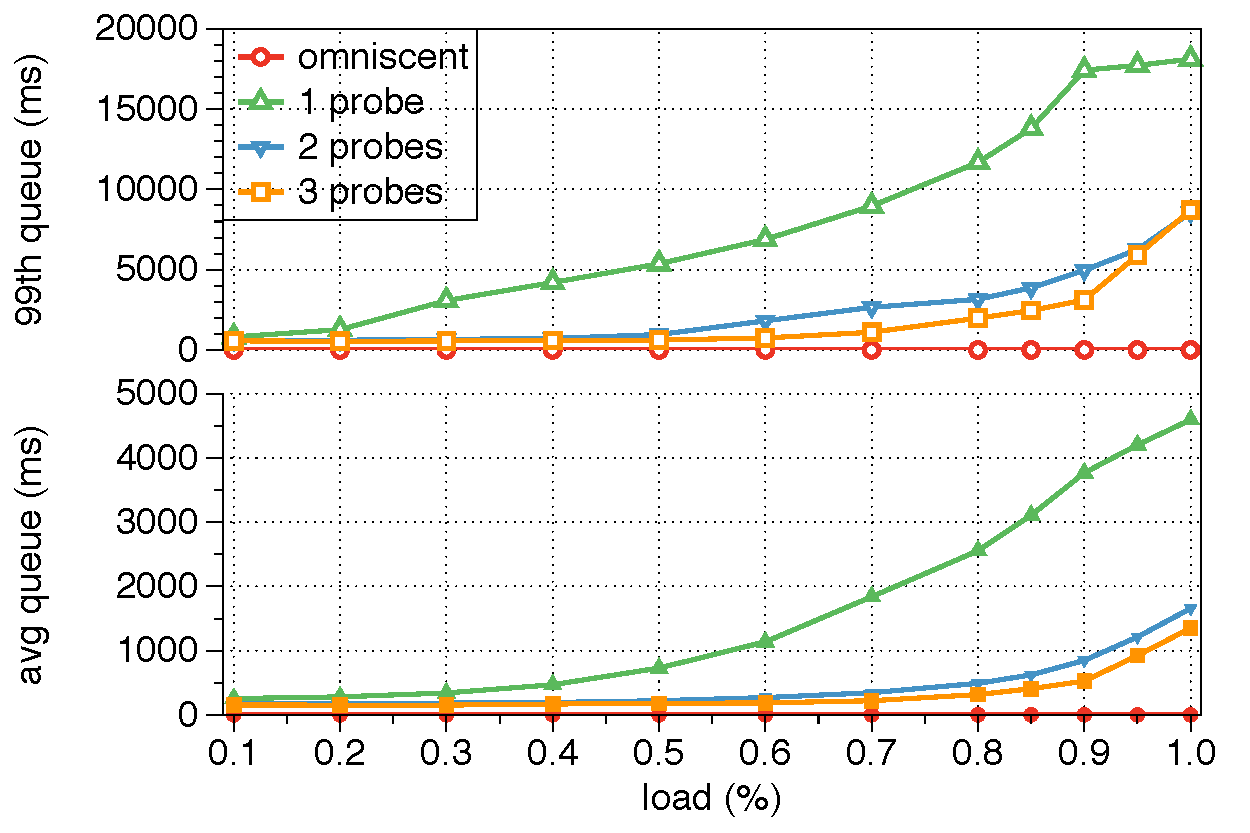
\includegraphics[width=.5\textwidth]{figures/probes_new}
  \caption{Base Sparrow algorithm using different load and number of probes}
  \label{fig:probes}
  \end{center}
  \end{figure}

  \begin{figure}
  \begin{center}
  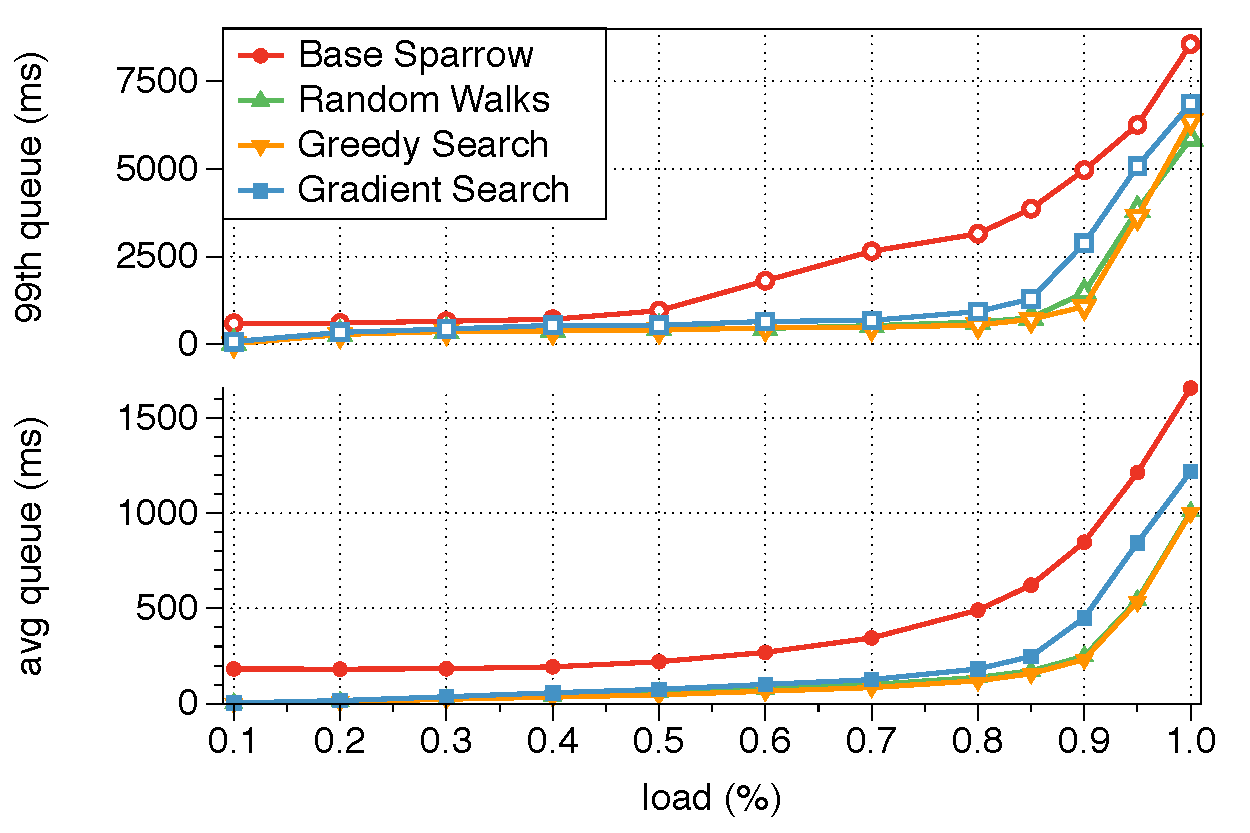
\includegraphics[width=.5\textwidth]{figures/comparison_new}
  \caption{Comparison between Base Sparrow Algorithm and its enhancements}
  \label{fig:comparison}
  \end{center}
  \end{figure}

  The comparison shows how the Self Assignment decreases the average queue
  time, since in most cases the task is not propagated at all but
  immediately executed on the \tmast.

  The Probe Propagation instead decreases dramatically the 99th percentile
  queue time, especially with loads between 50\% and 85\%, and similarly on
  all the configurations. Above 85\%, all configurations experience an
  increase in both average and 99th percentile. 

  Neither average nor 99th percentile obtain a significant improvement by
  using a Greedy Search on top of Random View.

  Finally the last configuration, using Gradient, performs slightly worse
  than the others. Although we did not verify this dynamics, our hypothesis
  is that the samples provided by Cyclon carry stale information about the
  neighbour resources. This results in the nodes on top of the gradient to
  receive an higher amount of probes. 

  The Gradient Ranking function seems to provide a very little improvement
  when the load increases too much. Intuitively this is because of the power
  of two choices, at least half of the of the place-holders could get a
  Cancel on confirmation request. Moreover, the use of the Late Binding
  technique further reduces the correlation between the length of the
  waiting queue and actual load.

\subsection{Results in Random Scenarios}

  \begin{figure}
  \begin{center}
  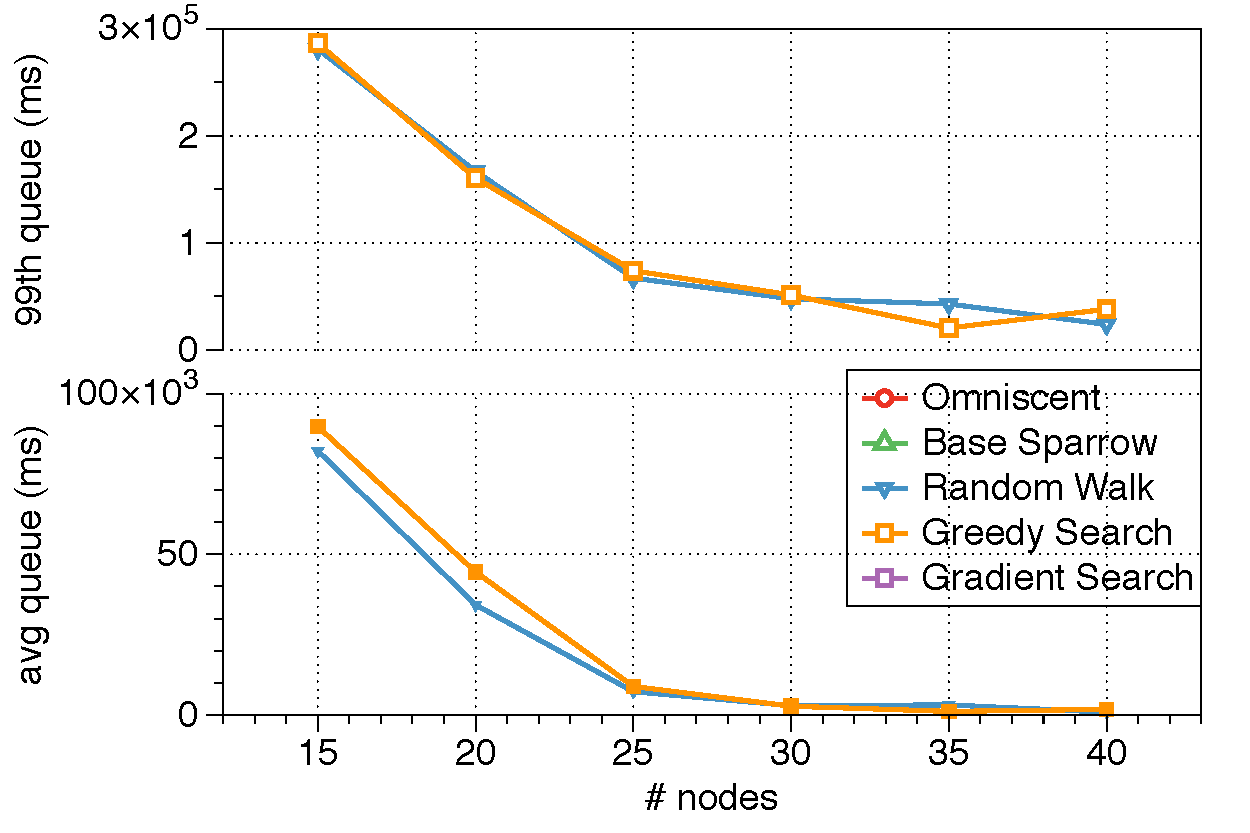
\includegraphics[width=.5\textwidth]{figures/randomA}
  \caption{Random Scenario A}
  \label{fig:comparison}
  \end{center}
  \end{figure}

  \begin{figure}
  \begin{center}
  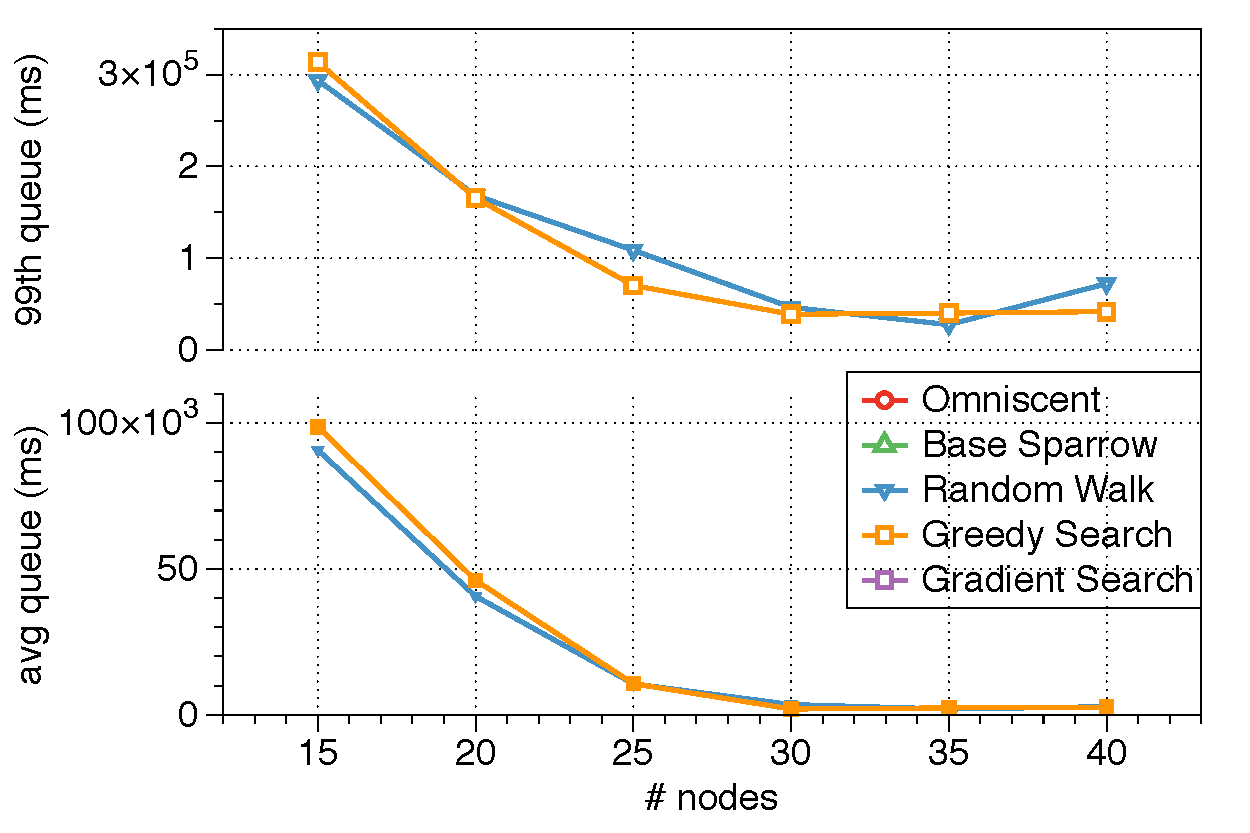
\includegraphics[width=.5\textwidth]{figures/randomB}
  \caption{Random Scenario B}
  \label{fig:comparison}
  \end{center}
  \end{figure}

  \begin{figure}
  \begin{center}
  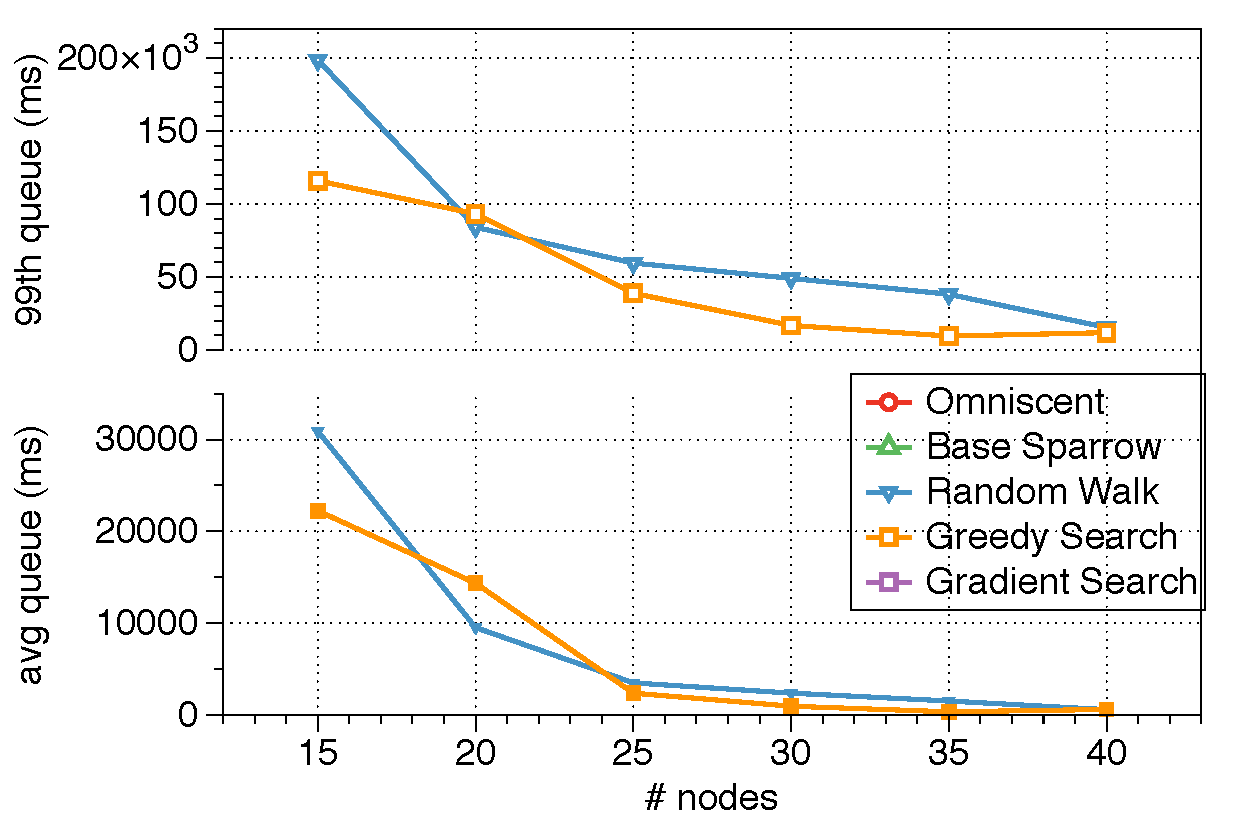
\includegraphics[width=.5\textwidth]{figures/randomC}
  \caption{Random Scenario C}
  \label{fig:comparison}
  \end{center}
  \end{figure}

  %The Random Scenarios show a similar trend with the load scenario, except
  %for the scenario C, with heterogeneous nodes, where Greedy Search helps to
  %decrease the queue time in the worst cases.  This is therefore the only
  %case, in our implementation, where a Greedy Search or Gradient gives
  %slightly better result. In case of node heterogeneity, the random walks
  %are sufficient to balance the load among all nodes

  The Random Scenarios show similar trends with the load scenario, with
  Greedy Search slightly decreasing the Random Walk performances. Only in
  the heterogeneous nodes scenario C the Gradient Search helps decrease
  the 99th percentile when there are enough resources available (more than
  25 nodes).
 
  Therefore, in all scenarios analysed for our implementation, Random
  Walks, and Greedy Searches gives better result than the base Sparrow
  algorithm.

  There are two main differences between using Random Walks and Greedy Searches:
  \begin{itemize}
    \item The cost of increasing the rate of Cyclon, aimed at providing
      fresh samples of the utility function;

    \item The development of a more complex utility function which takes
      into account more resources besides CPU and memory, possibly
      also improving the queue-time estimation when using Late Binding.
  \end{itemize}

\end{document}
